\section{Working with the RAW file format}
\label{sec:raw}

This section describes the structure of the "raw" format files generated by the usage of the HPCAP driver as explained in~\cite{MorenoTFM2012}.\\

RAW files are generated by the programs that fetch traffic from the network using the \texttt{HPCAP} driver (see~\ref{subs:samples}).


\subsection{File data structures}

A raw file is composed by a set of consecutive packets.
Each packet is preceded by its corresponding header which contains information related to the packet just as shown in \fref{fig:rawformat}:

\begin{itemize}
	\item \textbf{Seconds} 4 bytes containing the seconds field of the packet timestamp.
	\item \textbf{Nanoseconds} 4 bytes containing the nanoseconds field of the packet timestamp.
	\item \textbf{Caplen} 2 bytes containing the amount of bytes of the packet included in the file.
	\item \textbf{Len} 2 bytes containing the real size of the packet.
\end{itemize}


\begin{figure}[h]
	\centering
	\begin{center}
		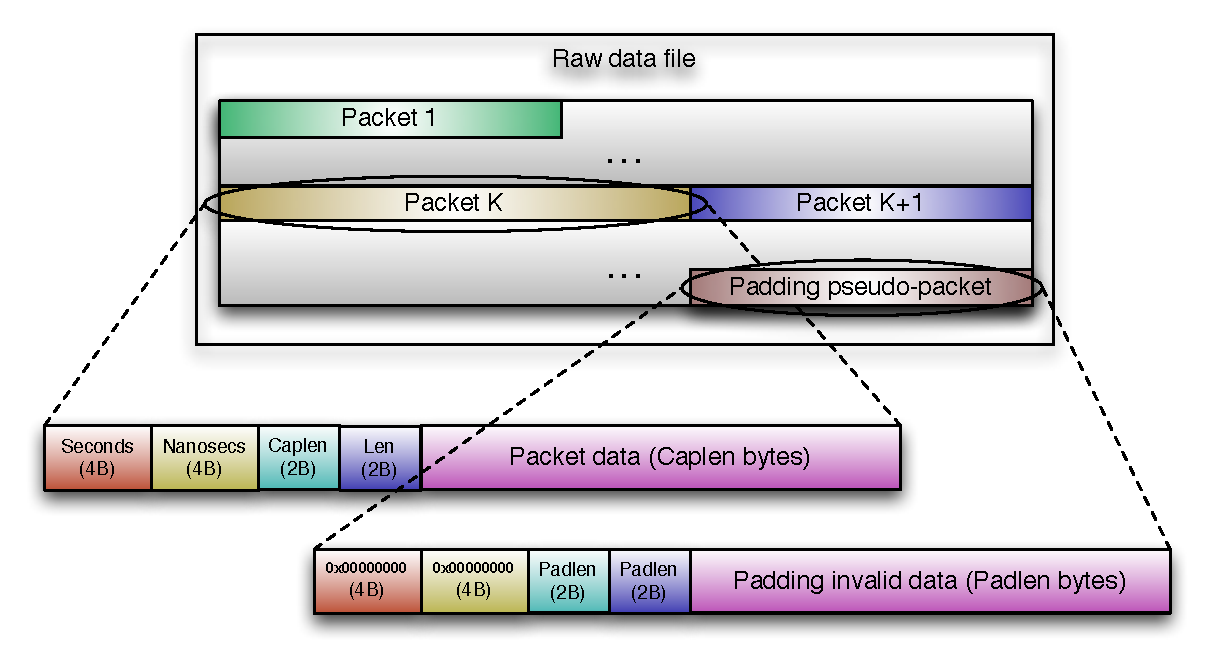
\includegraphics[angle=0,width=\textwidth]{figs/buff_raw2.pdf}
		\caption{Raw file format}
		\label{fig:rawformat}
	\end{center}
\end{figure}


The end of the file is denoted by the appearance of a pseudo packet showing the amount of padding bytes added at the end of the file (in order to generate files of the same size).
The padding pseudo-packet has a similar header than any other packet in the file with the difference that both the "Seconds" and the "Nanoseconds" fields are set to zeros.
Once the padding pseudo-packet has been located, the padding size can be read from any of the "Len" or "Caplen" fields. Note that the padding length could be zero.

\subsection{Example code}

The file \textit{raw2pcap.c} in the \textit{samples/raw2pcap} folder is an example of a program that reads a raw file and generates a new pcap file with the contents of the first one.



